\chapter{脉冲神经网络}
\label{chap:spiking-networks}

先从一种特殊的传感器说起。普通相机每隔固定时间拍下一整帧，无论画面有没有变化都要产生并处理一整张图；事件相机则完全不同，它只在某个像素的亮度发生变化时，才送出一个带时间戳的事件——“第几行第几列、在什么时刻、变亮还是变暗”。面对这样的输入，前几章那种“每隔一段时间吃进一个稠密实数向量”的网络就显得别扭：若等够一帧再处理，会白白浪费事件天然带有的精确到达时刻，把“哪次变化先到、哪次后到”的先后信息抹平；若每收到一个事件就重算整张图，又要对绝大多数根本没变的位置做无用功。于是自然产生一个问题：能不能让网络直接以“到达的事件”为基本输入，在处理事件的同时保住它们的强度、先后顺序和更早以前留下的影响？

这个问题的答案，就是本章要讨论的脉冲神经网络。信号在网络里不再以连续实数的形式传递，而是以一个个离散的“发放事件”传递；一个事件本身极其简单，只说明“某个单元在某个时刻发放了”，信息要靠事件的次数、到达的时刻以及单元内部保存的历史状态来共同承载。

生物神经元恰好就是这样通信的：细胞内部的膜电位连续地积累和消退，但神经元向远处发出的信号却是短促、离散的动作电位。液态状态机也已经用固定的脉冲储备池形成随时间演化的动态、再训练一个读出（见第\ref{chap:neural-network-overview}章与第\ref{chap:recurrent-networks}章）。但如果还想让多层连接都能从任务误差中学习，就必须回答：输入怎样编码成事件、单元内部怎样积累历史、连接怎样传播事件，以及最终误差怎样接回到这些离散事件和连续状态上。输入怎样编码，内部怎样积累，连接怎样传播，决定这种通信能完成什么预测；时间模拟与训练则产生相应成本。

阅读本章时可以始终抓住一对区分：单元对外传出的是离散脉冲（0或1的事件），单元内部保存的却是膜电位这样的连续状态。事件在到达的瞬间改变状态，两次事件之间状态仍按自己的规律继续演化，于是很久以前的输入也能影响此刻的响应。本章先用离散时间把连接输入、状态更新、学习和读出完整地串成一条计算路径，再用它解释“事件稀疏”到底在什么条件下才能真正省下计算；其中的连续时间方程则为这些离散更新提供物理与数学上的来源。

\section{脉冲神经网络概述}
\label{sec:snn-overview}

\subsection{提出动机与核心思想}
\label{sec:snn-motivation}

为什么要放着熟悉的实数激活不用，转而研究这种更“原始”的脉冲通信？动机来自生物现实和工程现实两端。生物细胞的膜电位在细胞内是连续变化的，但它向其他细胞远距离通信时，主要靠的是一个个短暂、形状几乎固定的动作电位（脉冲）；如果只用一个实数激活概括细胞的活动，单次发放发生在什么时刻、两次发放间隔多长、阈值以下还在悄悄积累了多少，这些信息就全被略去了。神经科学要解释细胞如何响应输入，就绕不开这些量；而事件相机这类变化驱动的传感器，又恰好直接提供了带精确时刻的观测。

\term{脉冲神经网络}（spiking neural network, SNN）以离散发放事件在单元之间传递信息，单元内部保存随时间演化的状态。一个脉冲通常只报告某单元在某时刻发放；信号的强度和时序关系由发放次数、发生时刻及发放单元共同承载。接收单元积累这些输入，旧输入逐渐衰减，状态越过阈值时再产生新事件。事件序列承担编码，阈值、复位与状态递推形成处理这些序列的网络。

需要强调的是，“用0和1通信”本身并不自动等于省电或更强大，这类模型真正服务的是两类不同的问题，评价方式也不同。神经科学需要用动态解释细胞的输入响应，以及局部连接怎样形成行为，关心的是模型是否符合生物证据；工程则希望在输入变化稀疏时，按到达事件传递和处理信息，减少持续感知中的操作，关心的是端到端的实际开销。后一收益取决于完整链路：传感器与编码到底产生多少事件，网络实际访问多少连接，设备又以什么方式更新状态。仅仅把通信变量取成0与1，并不能推出这些成本。

对本科阶段的工程任务，可以使用只保留积累、泄漏、阈值和复位四种机制的简化单元，通过任务损失学习连接参数，再用连续值读出形成预测——不必复刻真实神经元的全部离子通道。究竟保留哪些细胞机制，应由研究问题决定：解释发放过程需要相应的生物证据，分类需要任务评价，节省计算则需要检查实际执行的事件与状态更新。

\subsection{从神经元建模到神经形态计算}
\label{sec:snn-early-history}

脉冲网络的发展汇合了神经元动态、时序编码和硬件实现几条路线。它们分别解释事件怎样产生、时间怎样承载信息，以及事件怎样被执行。1907年Lapicque的积分发放思想将输入电流的积累与阈值发放联系起来，是早期简化动态模型的一条路线\scite{gerstner2014}

1952年Hodgkin与Huxley从离子电流出发建立动作电位的定量模型。与积分发放模型相比，它解释波形产生机制，说明神经元模型可以在不同生物细节层次上工作：简化模型便于组织较大网络，细致模型则服务于膜电流和发放机制研究\scite{hodgkin1952membrane}

1990年，Mead系统讨论\term{神经形态电子系统}（neuromorphic electronic systems），即借鉴神经系统组织与动态来设计电子计算系统。它关注的不仅是某个神经元方程，还包括局部连接、并行动态和物理实现；神经形态计算的范围因此比某一种SNN模型更广\scite{mead1990neuromorphic}

1997年，Maass以“第三代神经网络模型”讨论脉冲单元的计算能力，把发放时间明确纳入计算。这一代际划分比较阈值单元、连续激活与脉冲时序能够完成的计算。相应表达结论限定了编码和单元模型；实际任务精度与设备能耗还由训练、数据和执行方式决定\scite{maass1997spiking}

脉冲储备池进一步展示了利用复杂动态而不训练全部循环连接的路线。2002年的液态状态机让输入扰动一个固定循环系统，再训练读出使用其动态状态；第\ref{sec:rnn-lsm}节已给出这种分工。局部可塑性则从突触两端活动出发调整连接，为无需完整反向传播的学习提供另一条路径。储备池把可训练部分放在读出，局部规则把可用信号限制到突触附近；多层监督任务还需要把最终误差分配到更早的事件和连接。

\subsection{深层网络与训练方法的发展}
\label{sec:snn-learning-history}

当目标从解释局部动态转为学习多层分类器，离散阈值成为主要困难。2002年，Bohte等提出SpikeProp，根据发放时刻与目标时刻之间的误差进行反向计算；它对发放时刻求导，所需的模型与发放条件限定了这种时间误差回传的用法\scite{bohte2002spikeprop}

后来的两条路线让深度学习经验更容易进入SNN。一条先训练连续值网络，再校准权重和阈值，使脉冲统计近似原激活；另一条在前向保留离散发放，在反向指定替代导数，直接优化任务损失。第\ref{sec:snn-learning}节会分别说明转换误差和替代梯度的近似性质。2019年的替代梯度综述系统整理了后一条路线，替代规则为不连续发放提供了指定的反向信号，前向阈值仍然保留\scite{neftci2019surrogate}

可训练性改善后，研究开始扩展深度与信息交互方式。2021年的SEW-ResNet研究怎样在脉冲残差路径中保持合适的传播；2022年发布、2023年发表于ICLR的Spikformer则将脉冲形式的查询、键和值用于注意力计算。残差组织层间传播，注意力组织信息读取；其中连续运算、时间步使用和硬件映射方式又分别影响训练与执行成本\scite{fang2021spikingresnet}

Spikformer将两种约定组合起来：事件编码与神经元动态规定单元怎样响应，注意力与层间组织规定怎样读取信息。具体模块需要相应的脉冲实现；静态图像还需编码成多步输入，其事件数由这份编码与网络响应决定\scite{zhou2023spikformer}

\subsection{与连续值神经网络的比较}
\label{sec:snn-ann-comparison}

两类网络都可以有前馈、卷积、循环或注意力连接，所以SNN并不是一种全新的“拓扑”，它与普通网络的区别主要落在单元输出的形式和时间动态上。普通前馈单元一次前向就产生一个实数激活，计算结束后内部不留存东西；脉冲单元则先更新内部状态、再决定这一步是否发放，发放与否都是离散事件。即使没有任何循环边，漏积分发放（leaky integrate-and-fire, LIF）单元也能用膜电位把过去若干步的输入记住，而普通逐帧前馈网络通常没有跨帧状态——这一点和第\ref{sec:rnn-lsm}节的LSM呼应。RNN同样保存跨时间状态；SNN与之相比，特殊之处在于明确的阈值发放、发放后复位和以事件进行通信这三件事。

还要特别澄清一个容易混淆的点：同样是一个值为1的比特，在二值网络里它只是某层的离散输出，在SNN里它表示“某个时间区间内发生了一次发放”，含义与内部状态紧紧相连。脉冲单元这一步输出0，并不等于它什么都没“想”——过去的输入可能正悄悄积累在膜电位里，下一个事件到来时就可能叠加越过阈值而发放。表~\ref{tab:snn-ann-comparison}从通信、状态、时间、求导、训练、成本和读出几个方面系统比较两者。
\begin{table*}[htbp]
  \centering\small
  \begin{tabularx}{\linewidth}{@{}p{25mm}XX@{}}
    \toprule
    比较维度 & 连续值网络 & 脉冲神经网络 \\
    \midrule
    通信变量 & 实数激活或向量 & 发放事件；数量与时刻共同承载信息 \\
    单元内部状态 & 前馈单元通常无跨输入状态；RNN有状态 & 膜电位、突触响应及可选适应状态 \\
    时间关系 & 由递推、位置或时间特征表达 & 由事件时刻、积累、泄漏与延迟表达 \\
    求导困难 & 常见激活可微或分段可微 & 阈值发放不连续，需特别处理 \\
    训练路线 & 任务梯度及其他学习方法 & 局部规则、时间求导、替代梯度或网络转换 \\
    执行成本 & 取决于算子、稀疏性与设备 & 还取决于观察窗口、事件访问和状态更新 \\
    输出形式 & 分类分数、概率或连续量 & 计数、发放时间或连续状态读出 \\
    \bottomrule
  \end{tabularx}
  \caption{以常见人工模型比较两类网络。连续值网络也能使用稀疏计算、动态状态和局部学习；SNN也可能在通用设备上按固定时间步进行稠密计算。预测质量和能耗需要在相同输入、决策条件与设备设置下另作比较。}
  \label{tab:snn-ann-comparison}
\end{table*}
\FloatBarrier

\subsection{应用现状与发展方向}
\label{sec:snn-development}

事件视觉、稀疏声音或触觉感知、持续监测与机器人响应，是SNN值得研究的场景：输入随时间到达，变化可能稀疏，决策又关心响应延迟。2017年Amir等将事件相机、脉冲识别网络与TrueNorth处理器用于实时手势识别，给出了传感器到设备执行的完整研究系统。这项研究把事件输入、网络响应和设备测量接在同一链路中，结果对应其手势任务、设备与测试条件\scite{amir2017gesture}

硬件的发展提供了更灵活的实验平台。Loihi面向事件通信、神经元状态和片上学习；Loihi 2进一步支持可编程神经元动态。Intel于2024年公布并部署到Sandia的Hala Point，以Loihi 2构成大规模神经形态研究系统。这项交付为研究设施提供了较大规模的事件计算平台，应用范围由设施中的具体实验与工作负载界定\scite{intel2024halapoint}

应用前景取决于完整链路。若输入本来是密集静态图像，需要编码并模拟许多时间步，事件数量和等待时间可能抵消部分收益；若输入是稀疏事件流，输出还需在较短窗口内可靠形成，噪声、低发放量和阈值校准就更关键。分类结果衡量预测，操作量或能耗估计描述成本模型，实际设备测量则反映执行链路；共同的输入与决策条件使这些结果能够相互对应。

已有发展显示两条仍在推进的路线：一条扩大模型的可训练深度、注意力组织和任务范围，另一条围绕稀疏传感器与专用设备共同设计编码、动态和执行方式。深层任务模型与完整实验系统已经提供了可研究的计算对象。数据适配、训练成本、状态存储和软件执行决定这些对象怎样进入其他场景；后面的结构、学习与理论分析将把这些条件落到编码和动态上。

\section{网络结构}
\label{sec:snn-coding-dynamics}

脉冲网络由输入编码、带状态的神经元、突触连接和读出四部分组成。可以用一个问题串起它们：一个连续变化的外部世界，怎样变成网络能消费的事件（编码）；事件到达单元后留下什么、积累多久、何时再向外发出新事件（神经元动态）；新事件被送往哪些单元、延迟多久到达（突触连接）；最后怎样从一段时间的发放中读出答案（读出）。连接决定事件送到哪里，神经元动态决定事件到达后留下什么状态、何时产生下一次发放。输入编码规定事件含义，单元内部的计算规定历史保留；把这些单元接起来，才得到前馈或循环的信息路径。

\subsection{频率编码与时间编码}
\label{sec:snn-coding}

假设一个传感器在一段时间内观察到某种强度，比如光强是0.7。连续值网络可以直接把0.7这个数喂进去，脉冲网络却必须先回答一个全新的问题：实数0.7要怎样“翻译”成一串0和1的事件？这就是编码要解决的事。对第$i$个输入通道，记发放时刻为$t_{i,k}$。连续时间的脉冲列可以形式化为
\begin{equation}
  s_i(t)=\sum_k\delta(t-t_{i,k})\text{，}
  \label{eq:snn-spike-train}
\end{equation}
其中$\delta$为Dirac脉冲，其意义通过积分给出：对一个只包含某次发放的时间区间积分，得到1。这个表示省略了动作电位的波形，只记录事件时刻。计算机模拟常将时间分为宽度$\Delta t$的$K$个区间，令$s_i^{(t)}\in\{0,1\}$表示第$t$个区间是否发放；若同一区间允许多次发放，可以改用计数，后续计算也相应处理这份次数。

\term{频率编码}（rate coding）用观察窗口内的脉冲数量表示输入强弱：信号越强，发放越密。这是最直观的方案，因为在一段足够长的时间里数脉冲个数，恰好得到一个与强度成正比的连续量。若窗口长度为$T_{\mathrm{win}}=K\Delta t$，计数与频率为
\begin{equation}
  N_i=\sum_{t=1}^{K}s_i^{(t)},\qquad
  r_i=\frac{N_i}{T_{\mathrm{win}}}\text{。}
  \label{eq:snn-rate-code}
\end{equation}
因此，同样的脉冲数即使排列不同，也具有相同的窗口频率。将非负输入$x_i\in[0,1]$编码为每个区间独立以概率$x_i$发放，是一种教学上容易分析的随机方案。它满足$\mathbb E[N_i/K]=x_i$，方差为$x_i(1-x_i)/K$。延长窗口可以降低这种抽样误差，但增加等待时间和期望事件数。这里的方差来自独立抽样；相关发放的计数误差还会包含事件之间的协方差。

如果任务要区分“哪个信号先到”，仅统计数量就从根本上无能为力了——频率编码把脉冲在时间轴上打乱，只留下总数。很多实时任务关心的恰恰是先后：声音先到左耳还是右耳决定了声源方向，前方障碍先触发哪个传感器决定了运动趋势。于是需要另一种编码，让时间本身携带信息。\term{时间编码}（temporal coding）用发放时刻或相对时间关系承载信息。例如，\term{首次发放时间编码}（time-to-first-spike coding）可以约定强输入更早发放，在窗口起点已知时令$t_i=T_{\mathrm{win}}(1-x_i)$：输入越强，越早发出第一个脉冲，理论上一个事件就能区分很多强度等级。也可以用相邻脉冲间隔或多个单元的相对时序编码。首次发放的含义依赖窗口起点与时间到强度的约定。未发放如何解码、时间怎样量化，以及抖动和起点误差怎样影响恢复值，也属于这份编码。

图~\ref{fig:snn-codes}中的两组事件计数相同、顺序不同。频率读出把它们映射到同一个数；保留时刻的输入则让动态网络获得另一种区分依据。突触、状态和最终读出需要继续保留这份时序差别，它才会进入预测。
\begin{figure}[htbp]
  \centering
  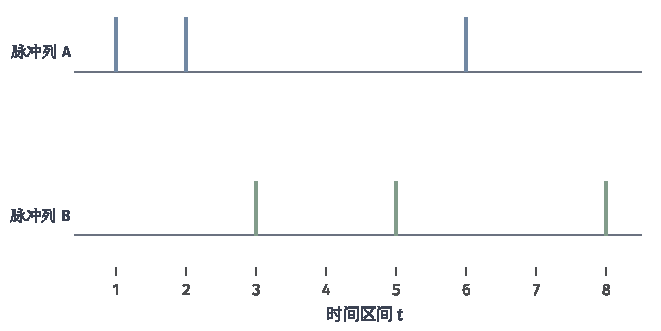
\includegraphics[width=105.412mm]{figures/05-neural-network-models/00-shared/matplotlib/snn-codes/figure.pdf}
  \caption{两条构造的脉冲列在8个等宽时间区间内都发放3次，窗口频率相同，但首次发放位置和脉冲间隔不同。竖线表示事件，横轴为时间区间编号；频率读出只保留计数，时间读出还可使用排列。}
  \label{fig:snn-codes}
\end{figure}

输入编码与输出解码不必相同。网络可以接收时间戳事件，再用输出计数分类；也可以接收持续电流，通过输出单元的首次发放作决策。输入到事件、输出到预测的两份约定共同规定了任务接口，相同观察条件下才有共同的精度与延迟口径。

\subsection{积分、泄漏与发放}
\label{sec:snn-neurons}

图~\ref{fig:snn-neuron-structure}将一个单元拆为突触响应、积分与泄漏、阈值检测和复位。输入事件只在到达时写入突触，突触响应与膜电位则保存连续值状态。输出脉冲反馈到复位路径，复位后的电位再经过一个时间步进入下一次积累；这条内部反馈使先前积累可以影响下一次响应，即使单元之间没有循环边。
\begin{figure*}[htbp]
  \centering
  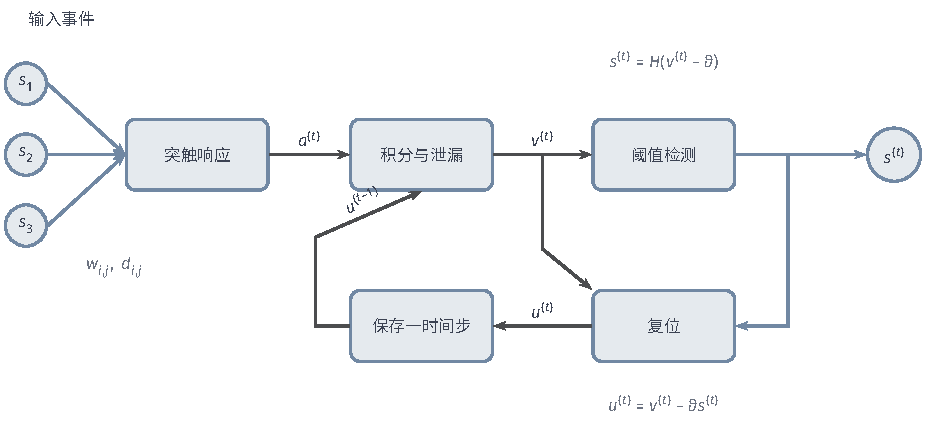
\includegraphics[width=156.792mm]{figures/05-neural-network-models/00-shared/tikz/snn-neuron-structure/figure.pdf}
  \caption{离散脉冲神经元的计算结构。输入事件经带权突触形成输入增量$a^{(t)}$，积分与泄漏模块更新复位前电位$v^{(t)}$，阈值检测模块输出脉冲$s^{(t)}$。复位模块计算电位$u^{(t)}$，下方反馈将其保存供下一步使用。图表示本章的更新次序，不表示细胞的解剖结构；突触自身也可保存状态，见式\eqref{eq:snn-synaptic-state}。}
  \label{fig:snn-neuron-structure}
\end{figure*}

一个输入脉冲通常不足以触发一次输出——否则单元只会机械地复制输入，谈不上“整合证据”。神经元真正有用的行为是：把陆续到达的输入一点点攒起来，在攒够之前保持沉默、对外只输出0，一旦积累越过某个门槛，就发出一个脉冲，然后清空（或部分清空）重新开始。同时，很久以前的输入不该和刚刚到达的输入同等重要，旧积累应当随时间慢慢淡去。为描述这套“攒—忘—发—清零”的机制，需要一个内部状态变量。\term{膜电位}（membrane potential）就是描述这种内部积累的状态变量。在简化人工模型中，膜电位相对于阈值的位置决定是否发放，这份积累还会影响下次响应。

\term{漏积分发放模型}（LIF）的名字正好概括了它的三件事：“积分”是把输入累加进膜电位，“漏”是让旧积累随时间泄漏衰减，“发放”是越过阈值时产生脉冲。它在两次发放之间用一阶动态描述积累与遗忘。设膜电位为$u_i(t)$，静息电位为$u_{\mathrm{rest}}$，输入电流为$I_i(t)$，膜时间常数为$\tau_m>0$，电阻为$R$，则
\begin{equation}
  \tau_m\frac{\mathrm d u_i(t)}{\mathrm d t}
  =-[u_i(t)-u_{\mathrm{rest}}]+RI_i(t)\text{。}
  \label{eq:snn-continuous-lif}
\end{equation}
无输入时，偏离静息电位的部分按$\exp(-\Delta t/\tau_m)$衰减。膜电位从下方达到阈值$\vartheta>u_{\mathrm{rest}}$时，模型产生一次脉冲并复位。\term{不应期}（refractory period）指发放后暂时不能再次发放的时间，可通过锁定状态或禁止发放来建模。微分方程描述两次发放之间的变化，阈值检测、复位和不应期再规定事件产生及其后的状态\scite{gerstner2014}

为便于训练，以下把静息电位移到0，并把电流及积分系数吸收到输入增量$a_i^{(t)}$中。这里的增量与膜电位具有相同单位，表示第$t$个时间区间内的输入折算到区间末端后留下的电位贡献。为了看清电流怎样变成这个量，先只考虑一个区间内没有发放的线性动态。旧电位衰减到区间末端；区间内各时刻的电流也分别积累，并按距离区间末端的时间衰减。因此，输入贡献为
\begin{equation}
  a_i^{(t)}=\frac{R}{\tau_m}
  \int_{(t-1)\Delta t}^{t\Delta t}
  \exp\!\left(-\frac{t\Delta t-\xi}{\tau_m}\right)I_i(\xi)\,\mathrm d\xi\text{。}
  \label{eq:snn-input-increment}
\end{equation}
积分中的$\xi$是连续时刻。越早到达的电流贡献经历的泄漏越久，这正是指数权重的作用。在这个区间积分的基础上，本章采用先积分、再在步末检测、再减去阈值的离散模型：
\begin{align}
  v_i^{(t)}&=\alpha u_i^{(t-1)}+a_i^{(t)},
  &\alpha&=\exp(-\Delta t/\tau_m),\label{eq:snn-discrete-integrate}\\
  s_i^{(t)}&=H(v_i^{(t)}-\vartheta),
  &H(z)&=\begin{cases}1,&z\geq0,\\0,&z<0,\end{cases}
  \label{eq:snn-discrete-fire}\\
  u_i^{(t)}&=v_i^{(t)}-\vartheta s_i^{(t)}\text{。}
  \label{eq:snn-soft-reset}
\end{align}
$v_i^{(t)}$为检测前电位，$u_i^{(t)}$为复位后电位，$\alpha\in(0,1)$控制相邻时间步之间的保留程度。此模型每步最多发放一次。若$v_i^{(t)}$远大于阈值，剩余电位会留到后面；这一单步表示因而无法记录步内可能出现的多次发放。时间步与输入尺度共同决定这项发放上限是否适合任务。

若区间内电流恒为$I_i^{(t)}$，式\eqref{eq:snn-input-increment}中的积分给出$a_i^{(t)}=R(1-\alpha)I_i^{(t)}$。例如，$\alpha=0.8$且$RI_i^{(t)}=3$时，本步输入增量为0.6；已有电位先保留原来的0.8倍，再加上这份输入。这个换算说明了输入增量与电流的关系，但步末检测仍是离散模型另作的约定，不会因区间积分精确就恢复所有步内发放时刻。人工离散网络也可以直接规定$a_i^{(t)}$，将输入尺度包含在连接权重中。后面令$\alpha=1$得到IF模型时，仍保留已规定的输入增量；这一步不再要求沿用上述有限时间常数LIF的恒流换算。

式\eqref{eq:snn-soft-reset}称为减法复位，保留超过阈值的剩余电位——它对应“一次发放只放掉恰好一个阈值那么多的电位”，因此一个很强的输入可以在后续步继续触发发放。另一种\term{硬复位}（hard reset）则更彻底，直接将发放后的电位设为$u_{\mathrm{reset}}$，即$u_i^{(t)}=(1-s_i^{(t)})v_i^{(t)}+s_i^{(t)}u_{\mathrm{reset}}$，等于每次发放后把积蓄全部清空。两种复位既改变前向轨迹，也改变反向传播。去掉泄漏、令$\alpha=1$，旧积累永不衰减，就得到离散的\term{积分发放模型}（integrate-and-fire, IF），它是后续“ANN转换”一节的理论基础；增加适应变量或非线性电位项，可以描述更丰富的发放模式。增加适应或其他动态状态，也增加相应的存储、更新与求导路径。

\begin{example}[相同输入在不同间隔下的结果]
  \label{ex:snn-integration}
  取$\alpha=0.8$、$\vartheta=1$、$u^{(0)}=0$，不设不应期。输入增量$(0.6,0.6,0,0.6)$依次给出检测前电位$(0.6,1.08,0.064,0.6512)$，输出为$(0,1,0,0)$，复位后电位为$(0.6,0.08,0.064,0.6512)$。第二步的两个近邻输入共同越过阈值，第四步到来时，先前积累已经衰减，所得电位仍在阈值下。

  若将相同的三个$0.6$改放在第1、3、5步，中间输入为0，则检测前电位依次为$0.6,0.48,0.984,0.7872,1.22976$，只有第五步发放。总输入不变，输出时刻却改变了。这组教学数值把泄漏与事件间隔的作用落实到可复算的状态轨迹。
\end{example}

图~\ref{fig:snn-lif}把示例的第一组输入画成轨迹。检测前电位用于判断发放，复位后电位成为下一步的初始状态，图中的标记也按这一次序区分。
\begin{figure}[!t]
  \centering
  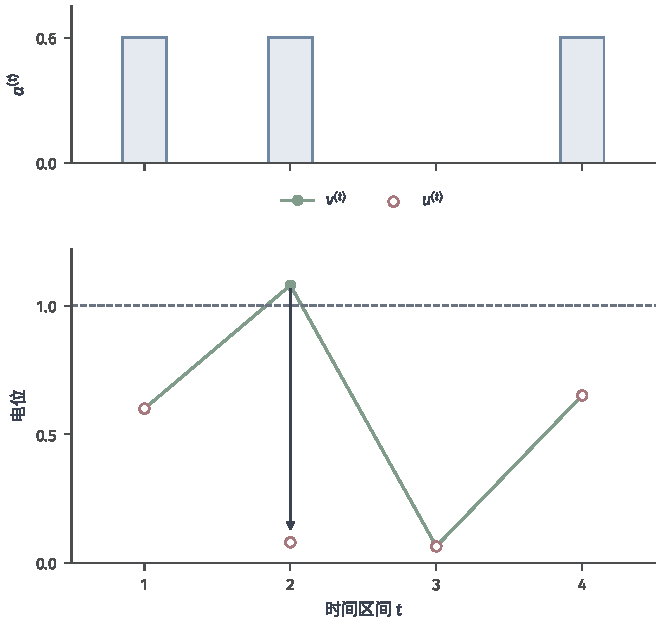
\includegraphics[width=105.412mm]{figures/05-neural-network-models/00-shared/matplotlib/snn-lif/figure.pdf}
  \caption{示例~\ref{ex:snn-integration}的离散LIF计算。蓝色柱形表示输入增量，绿色实线连接检测前电位$v^{(t)}$，红色空心圆为复位后电位$u^{(t)}$，虚线为阈值；第二步检测后发放并减去1。连线帮助比较离散状态，不表示步间的连续电位轨迹。}
  \label{fig:snn-lif}
\end{figure}

LIF保留了积累与遗忘，但它的阈值是固定不变的，这无法描述一种常见的“疲劳”现象：真实神经元在刚刚连续发放之后，往往会短暂地变得更难再次被激发，需要休息一会儿才恢复原有敏感度。固定阈值的模型只要输入不停就会一直按同一标准发放，体现不出这种自我抑制。要刻画它，可以让阈值随近期的发放历史而临时抬高，再随时间慢慢回落，这就是适应迹的作用。增加一个适应迹$r_i^{(t)}$，例如
\begin{equation}
  r_i^{(t)}=\rho r_i^{(t-1)}+s_i^{(t-1)},\qquad
  \vartheta_i^{(t)}=\vartheta_0+\kappa r_i^{(t)},
  \quad 0\leq\rho<1,\quad\kappa\geq0\text{。}
  \label{eq:snn-adaptive-threshold}
\end{equation}
这里$\vartheta_0>0$是基准阈值，$\kappa$决定适应迹对阈值的影响幅度。从无发放历史的初态开始时，可取$r_i^{(0)}=0$、$s_i^{(0)}=0$。若第$t$步发放，式\eqref{eq:snn-adaptive-threshold}会在第$t+1$步向迹中加入1；没有后续发放时，这次事件的贡献依次变为$1,\rho,\rho^2,\ldots$。当$\kappa>0$时，过去发放会暂时抬高阈值，适应迹随后衰减，阈值也逐渐回到基准。替换式\eqref{eq:snn-discrete-fire}中的阈值即可形成一种适应LIF模型。在这个示例中，复位仍按式\eqref{eq:snn-soft-reset}减去固定的$\vartheta$，可取$\vartheta=\vartheta_0$；若希望每次减去动态阈值$\vartheta_i^{(t)}$，则还需相应改变复位式。

额外状态增加了一条由$\rho$控制的发放历史通路，也增加反向路径和存储。它是否比原膜电位保留更慢的历史，要比较$\rho$与$\alpha$：在$\kappa>0$且$\rho>\alpha$时，一次发放在适应迹中的贡献比原电位的泄漏因子衰减得更慢，因而可以提供较长的响应时间尺度。若$\kappa=0$，这条迹不改变阈值；若$\rho=0$，它只保留紧邻前一步的发放。较慢的迹提供了保存历史的机制，能否据此完成需要长期信息的任务，还取决于输入、连接、学习和读出。

更复杂的神经元可以使用适应电流、非线性膜电位或离子通道状态。例如，\term{自适应指数积分发放}（adaptive exponential integrate-and-fire, AdEx）模型结合膜电位的指数非线性与适应电流。表~\ref{tab:snn-neuron-models}按状态变量与发放机制列出这些模型，使保留的细节与研究问题能够对应。
\begin{table*}[htbp]
  \centering\small
  \begin{tabularx}{\linewidth}{@{}
    >{\raggedright\arraybackslash}p{34mm}
    >{\raggedright\arraybackslash}p{49mm}
    >{\raggedright\arraybackslash}X@{}}
    \toprule
    神经元模型 & 主要状态与发放机制 & 适用关注点 \\
    \midrule
    积分发放（IF） & 膜电位积分，阈值与复位 & 简化计数对应，未包含泄漏 \\
    漏积分发放（LIF） & 膜电位积累与泄漏，阈值与复位 & 有限时间记忆与较低单元复杂度 \\
    适应LIF & 膜电位及适应迹，动态阈值或电流 & 发放历史改变后续响应 \\
    自适应指数积分发放（AdEx） & 膜电位非线性及适应电流 & 以较少状态描述丰富发放模式 \\
    Izhikevich模型 & 膜电位与恢复变量，阈值复位 & 以简化二维动态模拟多种放电行为 \\
    单室Hodgkin--Huxley & 膜电位与离子通道门控变量 & 解释动作电位产生的电流机制 \\
    \bottomrule
  \end{tabularx}
  \caption{神经元模型按保留的动态细节比较。IF与LIF还需规定复位、不应期及时间离散化；表中不计另行添加的突触和延迟状态。增加状态可以描述更多动态细节，任务预测质量则由数据、训练和相应读出评价。}
  \label{tab:snn-neuron-models}
\end{table*}
\FloatBarrier

模型细节由需要解释的响应决定。积累事件形成分类分数可以使用简化状态；研究动作电位波形或离子电流则需要能够产生这些量的动态。不同模型的参数单位、输入尺度与离散步长共同决定实际轨迹，相应数值要在各自方程中解释\scite{gerstner2014}

\subsection{网络连接与状态传播}
\label{sec:snn-connections}

图~\ref{fig:snn-connections}比较相同单元的两种组织。前馈边将事件送到下一层，每个单元的膜电位仍跨时间保留；循环边再把网络过去的发放送回当前计算。层间拓扑决定事件送往哪里，内部状态递推决定事件的影响保留多久，两者可以分别设计。
\begin{figure*}[htbp]
  \centering
  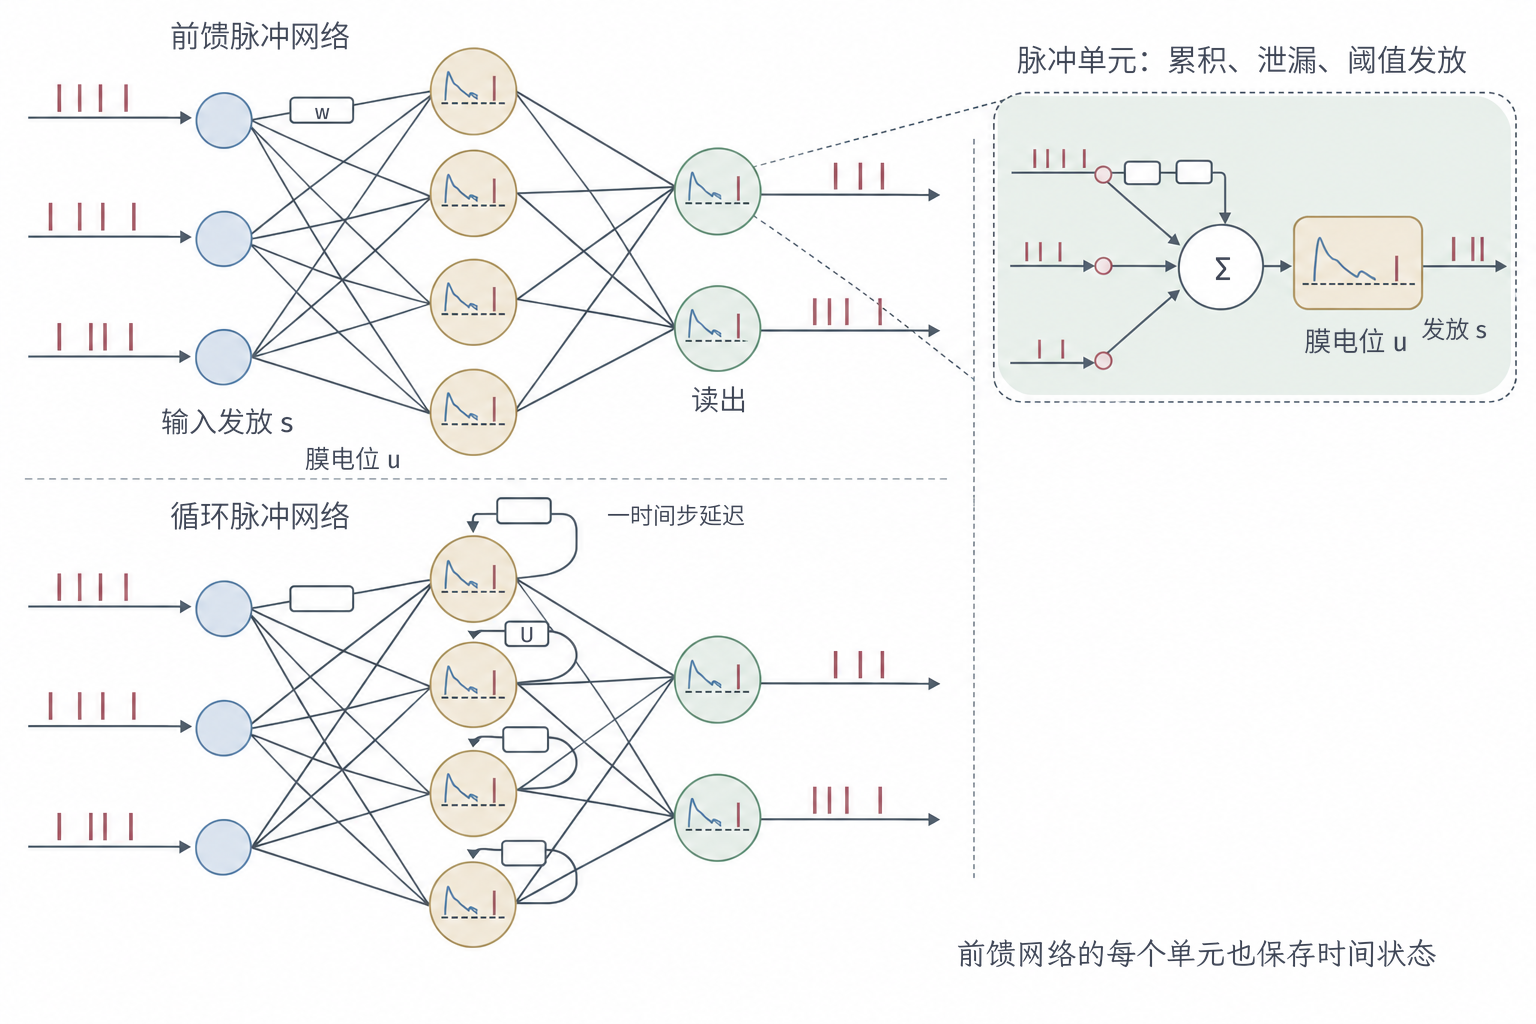
\includegraphics[width=130.048mm]{figures/05-neural-network-models/00-shared/generated/snn-connections/figure.png}
  \caption{脉冲前馈网络与循环网络的构造性比较。单元内的膜电位轨迹表示内部状态，箭头传递离散发放，右侧给出输出读出。上半部只保留层间前馈连接；下半部增加使用上一时间步脉冲的循环边$\bm U$。边还可带权重与传播延迟，图中只标出一条代表连接。神经元数和连边用于说明结构，不对应训练模型。}
  \label{fig:snn-connections}
\end{figure*}

神经元之间的连接把一个单元的发放变成其他单元的输入，这条连接在生物学上称为突触。在这里，\term{突触}（synapse）指带权连接及其对接收状态的作用，可以把它类比成前几章里带权重的连接边，但它传递的是离散事件而非连续激活。最简单的离散突触把一个到达脉冲转为电位增量$w_{i,j}$：每来一个脉冲，接收单元的膜电位就改变$w_{i,j}$这么多，正权重促使它接近阈值（兴奋性），负权重使其远离阈值（抑制性）。这里的人工模型允许同一单元的输出连接分别取正负权重。生物兴奋性、抑制性细胞对连接符号有更强约束，研究细胞类型时需将这些约束纳入模型。

为什么突触本身还需要状态？因为一个脉冲对接收细胞的影响往往不是瞬时的——生物突触释放的化学物质会让接收侧的电位在接下来一小段时间里持续变化，单个事件的作用会拖一个“尾巴”，多个事件的尾巴会叠加。要建模这种延续效应，突触就得有自己的状态变量。设一层有$m$个神经元，上层有$d$个，突触状态为$\bm q^{(t)}\in\mathbb R^m$，前馈权重为$\bm W\in\mathbb R^{m\times d}$，循环权重为$\bm U\in\mathbb R^{m\times m}$，偏置为$\bm b\in\mathbb R^m$，可写为
\begin{equation}
  \bm q^{(t)}=\beta\bm q^{(t-1)}
    +\bm W\bm s_{\mathrm{in}}^{(t)}
    +\bm U\bm s^{(t-1)}+\bm b,\qquad
  \bm a^{(t)}=\bm q^{(t)}\text{，}
  \label{eq:snn-synaptic-state}
\end{equation}
其中$\beta\in[0,1)$控制突触响应的衰减。到达脉冲写入$\bm q^{(t)}$，随后它与$\bm u^{(t)}$按各自衰减率保存历史。循环读取上一时间步的发放，使本步更新有已知输入；前馈层按层次顺序读取本步已经算出的发放。

更一般地，信号沿轴突传导需要时间，不同连接的延迟也不同，因此一个事件不一定要在下一个时间步立刻到达，可以让它“在路上走”若干步。引入延迟还有一个数学上的硬性理由：若允许零延迟的反馈环（包括自反馈），网络在同一时间步就可能出现自相矛盾的多个解，无法按确定顺序求值。令$d_{i,j}\in\{0,1,2,\ldots\}$表示边$j\to i$的总传播延迟，以离散时间步计，实际延迟为$d_{i,j}\Delta t$。权重为$w_{i,j}$的边贡献$w_{i,j}s_j^{(t-d_{i,j})}$；式\eqref{eq:snn-synaptic-state}中的前馈边对应$d_{i,j}=0$，循环边对应$d_{i,j}=1$。为保持显式更新，每个反馈回路的总延迟必须至少为一步；零延迟边组成的子图必须无环，才能按拓扑顺序读取本步已经算出的脉冲。若允许零延迟自反馈，例如$s=H(2s-1)$，则$s=0$与$s=1$都满足方程，同一历史因而允许两个本步输出，显式求值缺少唯一结果。实现还需维护尚未到达的事件队列，并为序列起点以前的脉冲指定初始历史。

脉冲前馈网络通过单元内部状态把当前响应接到历史输入上。加入循环边后，状态既保存本单元的积累，又接收其他单元的历史发放。初始状态、序列边界、延迟和同时到达事件的处理次序都属于模型定义；独立样本常重置状态，持续流则通常保留状态。

\subsection{观察时间与事件计算量}
\label{sec:snn-cost}

时间离散化和编码共同决定可表示的精度，这中间有一个绕不开的“精度—延迟”权衡。若用$K$步中的脉冲比例表示$[0,1]$内数值，能区分的最小间隔只有$1/K$：想让读数更精细，就必须观察更多步、等待更久；随机编码还叠加抽样方差。首次发放编码可以只用一个事件表示多个时间位置，理论上很快就能决策，但接收端必须一直等到该事件发生，并且要能区分事件落在哪个位置。事件较少可以降低相应通信量，较早决策则需要在更短观察时间内获得足够证据，这两者通常不可兼得。

\term{事件驱动计算}的省账方式和稠密矩阵完全不同，关键在于“只为真正发生的发放付费”。设一次推理中神经元$j$发放$N_j$次，连接到$d_j$个接收突触，若每次发放都访问这些连接，则触发的突触累加数为
\begin{equation}
  C_{\mathrm{syn}}=\sum_jN_jd_j\text{。}
  \label{eq:snn-event-cost}
\end{equation}
这个公式提醒我们：单靠“发放少”并不一定省。真正计入成本的是发放次数乘上扇出——一个单元即使很少发放，只要它的输出连接很多，每次发放仍要触发大量突触累加；反过来，一个孤立的高频单元影响的连接很少，开销也有限。除事件访问外，按时间步模拟$m$个状态单元本身还需要$O(Km)$次状态更新，因为即使没有输入，膜电位的泄漏、内部自发发放也要照算；若在通用硬件上实现为稠密矩阵乘法，未发放的那些零连接也未必会被跳过。事件驱动实现可以在到达事件时只更新相关状态，更贴合“为发生的事付费”，但它仍需额外处理泄漏、内部发放和延迟队列，工程实现并不免费。

所以，评价一个脉冲网络是否真的高效，必须算整笔账：既有事件访问，也有状态更新、延迟队列和存储管理。任务质量与决策延迟规定输出是否可用；突触访问和状态量描述成本来源，设备测量给出整条执行链的能耗。固定输入预处理与决策条件后，才能比较稀疏活动、连接组织和硬件执行各自带来的收益——这也解释了为什么在普通GPU上稠密模拟SNN常常并不省电。



\section{参数学习}
\label{sec:snn-learning}

有了网络结构，还必须解决学习问题：连接权重该怎么调，输出才能符合任务？对普通可微网络这靠反向传播，但脉冲网络里发放是阈值阶跃，在发放点不可微，这道障碍催生了三条思路截然不同、动机也各异的路线。第一条绕开梯度，直接模仿生物突触的局部规律：只用突触两端在时间上挨得近不近、谁先谁后来调整连接，不需要知道最终答案对错，也不需要全局反向传播。第二条正面迎上不可微：前向计算老老实实地用离散阶跃（保住脉冲的二值性和稀疏性），反向传播时则“善意地”把阶跃导数替换成一个光滑的替代导数，从而仍能做端到端梯度下降。第三条干脆不在脉冲网络里直接训练：先训练一个普通的连续值网络，再把它的实数激活解释成发放率，通过尺度校准转换成脉冲网络，复用已经学好的权重。三条路线使用的信息不同：局部规则根据相邻活动更新突触；端到端训练根据任务损失调整参数；转换方法先学习连续值网络，再把它的激活解释为脉冲统计量。它们可以组合使用，各条路径仍有自己的优化对象和误差来源。

下面的基本例子把泄漏、阈值和时间常数视为已给定参数，主要学习连接权重与读出。这些动态量其实也可以学习，例如用Sigmoid参数化泄漏因子、用正值变换参数化阈值，以维持模型约束；动态参数的梯度沿对应状态路径传播；整数延迟的改变则直接移动事件到达步，需要搜索或相应的可微近似。

\subsection{基于局部活动的突触学习}
\label{sec:snn-plasticity}

\subsubsection{基于共同活动的赫布更新}
\label{sec:snn-hebb-learning}

先看最简单的局部规则，它的动机是一个直观的因果联想：如果两个神经元总是在同一段时间里一起活跃，它们之间的连接多半是有用的，应当加强。这种规则完全不需要标签或全局误差，每个突触仅凭自己两端的局部信息就能更新，因而在硬件上极易分布式实现。\term{赫布学习}（Hebbian learning）根据输入端与输出端的共同活动调整连接，表达“共同活跃时加强联系”的局部相关性思想。一个简化规则为$\Delta w_{i,j}=\eta x_jy_i$，其中$x_j,y_i$是同一观察窗口的活动量，$\eta>0$为更新系数。它的隐患也很明显：持续相关活动可能令权重只增不减、无限增大，因此通常还需衰减、归一化、竞争或上下界。

\subsubsection{基于发放时间差的突触更新}
\label{sec:snn-stdp-learning}

但“共同活跃”还漏掉了因果方向。突触前（输入）先发放、突触后（输出）紧接着发放，说明前者很可能“促成”了后者，应当加强这条连接；反过来，输出已经发了、输入才到，那这次输入显然不是原因，反而应当减弱。把这种时间先后纳入权重更新，就能从单纯的相关走到带方向的因果。\term{脉冲时序依赖可塑性}（spike-timing-dependent plasticity, STDP）进一步依据突触前后发放的时间差更新权重。令$\Delta t=t_{\mathrm{post}}-t_{\mathrm{pre}}$，一种典型的成对教学规则为
\begin{equation}
  \Delta w_{i,j}=\begin{cases}
    A_+\exp(-\Delta t/\tau_+),&\Delta t>0,\\
    -A_-\exp(\Delta t/\tau_-),&\Delta t<0,
  \end{cases}
  \label{eq:snn-stdp}
\end{equation}
其中$A_+,A_->0$为幅度，$\tau_+,\tau_->0$为时间尺度，同时发放时另定规则。该形式把“输入先到、输出随后发生”与相反次序区分开。生物实验中的权重变化还随细胞类型、突触强度和发放组合改变\scite{bi1998}

局部计算不必保存所有事件对。可以用指数衰减的活动迹记录近期发放，突触后发放时读取突触前迹来加强权重，突触前发放时读取突触后迹来减弱权重。采用所有配对还是最近邻配对、权重是否有界，会产生不同学习动态。

\subsubsection{用任务信号调制局部更新}
\label{sec:snn-modulated-learning}

局部规则有个根本缺陷：它衡量的只是“两个单元是否经常一起发”，这与“它们是否有助于答对任务”是两回事——经常同时出现的输入可能只是背景噪声，真正区分类别的特征反而不那么频繁。要弥合这道鸿沟，需要让最终的任务结果（奖励或误差）也参与更新，哪怕它比局部事件晚到很久。生物大脑里多巴胺等神经调质正是扮演这种“全局广播的奖惩信号”：突触先把“我刚才活动过”记成一笔会随时间消退的账，等奖励到来时再据此决定加强还是减弱。为把局部活动与任务结果连接，可加入第三个调制信号，令$\Delta w_{i,j}=\eta m^{(t)}e_{i,j}^{(t)}$。其中$e_{i,j}^{(t)}$是记录近期局部活动及可更新程度的\term{资格迹}（eligibility trace），$m^{(t)}$传递奖励、误差或其他全局调制。迹保存的是哪些突触近期发生了可参与更新的活动，调制信号再决定这些活动应引起怎样的权重变化。第三因素由此把任务结果接到近期局部活动上，也允许任务信号比局部事件更晚到达。

第\ref{chap:neural-network-overview}章已经说明局部活动可以先留痕迹、等待奖励到来；现在可以把这段时间关系接到更新式上。作为一个示意构造，设$g_{i,j}^{(t)}$为第$t$步由突触两端活动形成的局部量，例如成对发放产生的带符号更新量，令
\begin{equation}
  e_{i,j}^{(t)}=\lambda_e e_{i,j}^{(t-1)}+g_{i,j}^{(t)},
  \qquad 0\leq\lambda_e<1\text{。}
  \label{eq:snn-eligibility-example}
\end{equation}
这里$\lambda_e$决定痕迹保留多久。假设第1步结束时迹为0，即$e_{i,j}^{(1)}=0$，第2步的局部活动使$g_{i,j}^{(2)}=1$，其后到第5步都没有新的局部量，那么第5步仍有$e_{i,j}^{(5)}=\lambda_e^3$。若任务调制此时到达，该步权重变化为$\eta m^{(5)}\lambda_e^3$。局部事件发生时先记录，之后逐步衰减，较晚的任务结果再读取尚存的迹；这三步解释了更新式怎样连接先前活动与后来结果。具体学习规则可以采用不同的资格迹，式\eqref{eq:snn-eligibility-example}只展示保留和调制的分工。只有相应调制信号与资格迹构造给出目标梯度时，才能据它作梯度下降分析\scite{gerstner2018plasticity}

\subsection{基于替代梯度的端到端学习}
\label{sec:snn-surrogate}

\subsubsection{离散发放的反向信号}
\label{sec:snn-surrogate-signal}

局部规则虽然省、也贴近生物，但它没有直接优化任务损失，难以和前几章成熟的深度训练接轨。最直接的监督学习做法，是像RNN一样把网络沿时间展开、用输出误差对所有连接做反向传播。先规定输出怎么读：设每个样本含$K$步输入脉冲，标签为$y$，输出读出为$\bm z=K^{-1}\sum_t\bm s_{\mathrm{out}}^{(t)}$，即统计输出单元在整段时间的平均发放率，可以用$\ell(\bm z,y)$训练分类器。膜电位、过滤状态或发放时间也可以形成预测；所选读出决定误差从哪些输出与时刻进入网络。

真正的拦路虎是式\eqref{eq:snn-discrete-fire}里的阶跃函数$H$：它在阈值以下和以上的普通导数都是0，只在阈值那一点跳变。如果老老实实地把这个导数代入链式法则，会发生两件糟糕的事——绝大多数位置的梯度都是0，误差根本传不回去，无法调整参数；而当某个参数只变一点点、让膜电位恰好跨过阈值时，输出又会从0突然跳到1，整条时间轨迹随之突变。\term{替代梯度}（surrogate gradient）用一个“前向照实、反向做手脚”的办法绕开它：前向计算中保留离散发放（输出仍是真实的0/1，保住脉冲的全部性质），在反向计算中则用一个有限、非零的光滑函数代替阶跃导数，给梯度开一条可通行的路。例如，令$z=v-\vartheta$，使用
\begin{equation}
  \frac{\partial s}{\partial v}\ \rightsquigarrow\
  \psi(z)=\frac{c}{(1+\kappa|z|)^2},\qquad c,\kappa>0\text{。}
  \label{eq:snn-surrogate-derivative}
\end{equation}
符号$\rightsquigarrow$标出反向所采用的规则，它与前向阶跃的普通导数承担不同角色。在固定$c$和$\kappa$时，$\psi$在阈值附近取较大的值，离阈值越远则越小。回传到电位的信号还要乘以从后续计算传来的误差；在其余回传量相同时，较大的局部替代系数才使这条路径保留较大的信号幅值。若后续传来的误差为0，即使电位靠近阈值，这条路径也没有回传贡献。因此，这里比较的是局部因子，不能仅按阈值距离判断完整参数梯度的大小。$c$改变梯度幅度，$\kappa$改变有效宽度；两者与阈值及电位尺度有关\scite{neftci2019surrogate}

替代规则也进入复位的导数。对本章的减法复位，若不停止复位路径的求导，有
\begin{equation}
  \frac{\partial u_i^{(t)}}{\partial v_i^{(t)}}
  \ \rightsquigarrow\ 1-\vartheta\psi(v_i^{(t)}-\vartheta)\text{。}
  \label{eq:snn-reset-gradient}
\end{equation}
若实现中把复位脉冲视为常数，这个导数改为1。两种约定共享前向轨迹，却给历史状态分配不同的回传信号；硬复位也按自身表达式产生另一组导数。复位路径的选择与发放处的替代函数共同组成训练规则。

图~\ref{fig:snn-surrogate-forward-backward}将真实前向发放与指定的反向规则放在同一计算链上。两种复位导数约定共享前向状态更新，区别只进入回传。

\begin{figure*}[htbp]
  \centering
  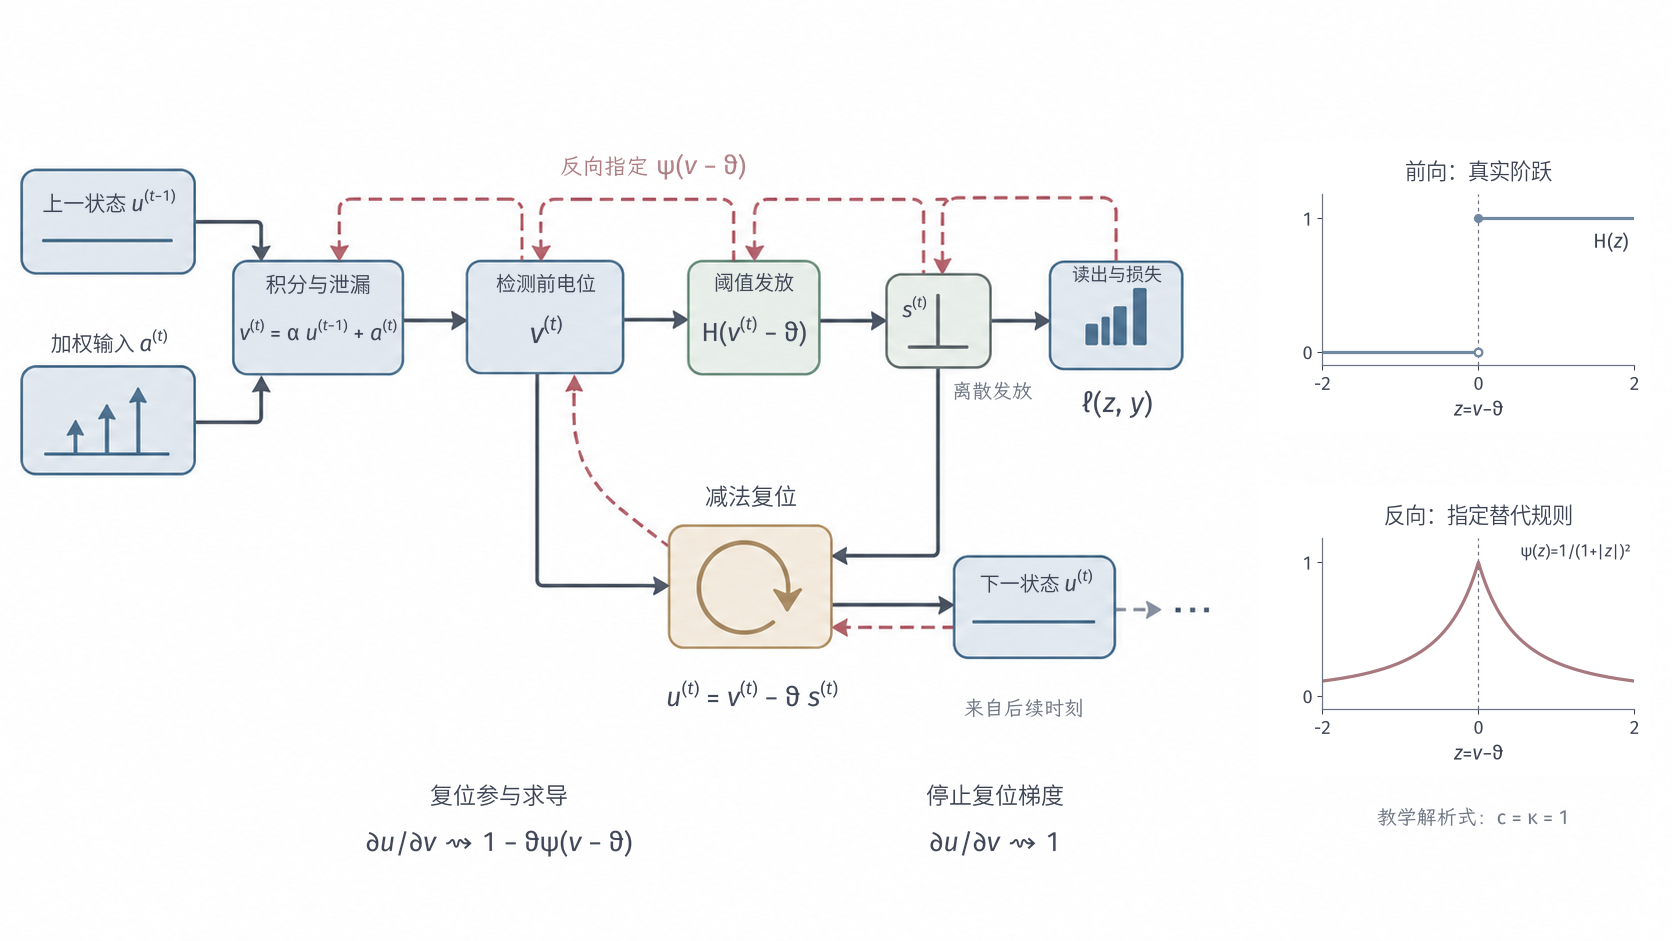
\includegraphics[width=141.563mm]{figures/05-neural-network-models/00-shared/generated/snn-surrogate-forward-backward/figure.png}
  \caption{LIF前向计算与替代梯度。前向使用真实阶跃发放和减法复位；反向在发放处指定替代规则$\psi$。右侧解析曲线取$c=\kappa=1$，阶跃在零处取一；下方两式分别表示复位参与求导与停止复位梯度，两种约定不改变前向发放。}
  \label{fig:snn-surrogate-forward-backward}
\end{figure*}

\subsubsection{沿时间展开分配任务误差}
\label{sec:snn-unrolled-training}

将$\bm q^{(t)}$、$\bm u^{(t)}$和所需延迟状态合并为$\bm h^{(t)}$，网络可写为$\bm h^{(t)}=F_{\bm\theta}(\bm h^{(t-1)},\bm x_t)$。这里$\bm h^{(t)}$表示第$t$步结束后保存的状态，包括供下一步读取的本步发放$\bm s^{(t)}$以及尚未到达的事件；更新第$t$步时，读取的则是$\bm h^{(t-1)}$中保存的历史。把这一递推展开到各个时间步，再累积所有调用同一参数的贡献，就得到第\ref{chap:recurrent-networks}章的时间反向传播；发放与复位处使用上述指定导数。

可以先沿一条膜电位路径看这种回传怎样发生。固定本步输入增量$a_i^{(t)}$、泄漏因子和阈值，只追踪$u_i^{(t-1)}\to v_i^{(t)}\to u_i^{(t)}$：旧电位先乘$\alpha$进入积分，再经过减法复位。将式\eqref{eq:snn-discrete-integrate}的局部系数与式\eqref{eq:snn-reset-gradient}相乘，这条直接路径的反向系数为
\begin{equation}
  \left.\frac{\partial u_i^{(t)}}{\partial u_i^{(t-1)}}\right|_{a_i^{(t)}\,\mathrm{fixed}}
  \ \rightsquigarrow\
  \alpha\left[1-\vartheta\psi(v_i^{(t)}-\vartheta)\right]\text{。}
  \label{eq:snn-membrane-backward-path}
\end{equation}
若停止复位脉冲的求导，这条路径的系数就变为$\alpha$。在更长的展开图中，同一路径沿时间继续传递时，会依次乘上各步相应的系数；循环突触、输出读出和其他状态还会形成额外路径，其贡献需要在汇合处相加。因此，式\eqref{eq:snn-membrane-backward-path}只展示直接膜状态路径，不是整个网络状态的完整雅可比。各时间步重复调用同一权重，最后仍须把这些调用位置对该权重的贡献累积起来。

在保存前向激活的实现中，较长窗口需要保存更多状态，重算可以改变这份存储代价；截断展开则删除相应历史梯度路径。所得回传信号由整套替代规则定义，其下降行为需要结合实际离散损失检验；对统一平滑目标作优化分析，还需另行建立这种规则与目标梯度的关系。

\begin{algorithm}[脉冲网络的监督训练]
  \label{alg:snn-supervised}
  \begin{algorithmic}[1]
    \Require 输入序列与标签、时间步数$K$、神经元参数、替代规则$\psi$
    \Ensure 学得的权重与读出参数
    \For{每个训练小批量}
      \State 按样本边界设置膜电位、突触状态和延迟队列
      \For{$t=1,\ldots,K$}
        \State 计算突触输入，按式\eqref{eq:snn-discrete-integrate}--\eqref{eq:snn-soft-reset}更新各层
        \State 保存反向计算所需状态并积累输出读出
      \EndFor
      \State 由读出与标签计算损失
      \State 沿展开图反向计算，以$\psi$代替发放导数并采用约定的复位导数
      \State 累积共享参数梯度，必要时裁剪，再更新参数
    \EndFor
  \end{algorithmic}
\end{algorithm}

\subsection{基于连续值网络的参数转换}
\label{sec:snn-conversion}

\subsubsection{连续激活与发放率的对应}
\label{sec:snn-rate-conversion}

第三条路线的动机很实际：替代梯度虽然能训，但脉冲网络仍然比普通网络难训得多、精度常常差一截，而连续值网络经过多年发展已有成熟的训练方法和大量高精度模型。能不能先把连续网络训到最好，再“无损地”搬到脉冲硬件上运行？这就需要建立一座桥梁：把连续网络里某个单元的实数激活，解释成脉冲单元在一段时间里的平均发放率——激活越大，对应单元发放越频繁；只要观察窗口足够长，发放率就能逼近那个实数。\term{人工网络到脉冲网络转换}（ANN-to-SNN conversion）就是建立连续激活与脉冲统计量的对应，以复用已经学得的权重。这座桥为什么成立、误差又从哪里来，可以从不泄漏的积分发放模型看起。

设$\alpha=1$、$u^{(0)}=0$，采用减法复位，每步输入增量为$a^{(t)}$，将$K$次状态更新求和得
\begin{equation}
  \vartheta\sum_{t=1}^{K}s^{(t)}
  =\sum_{t=1}^{K}a^{(t)}-u^{(K)}\text{。}
  \label{eq:snn-conversion-balance}
\end{equation}
若输入非负且每步不超过$\vartheta$，则$0\leq u^{(K)}<\vartheta$，于是
\begin{equation}
  0\leq\frac1K\sum_{t=1}^{K}a^{(t)}
       -\frac{\vartheta}{K}\sum_{t=1}^{K}s^{(t)}
  <\frac{\vartheta}{K}\text{。}
  \label{eq:snn-conversion-error}
\end{equation}
这说明阈值乘以平均发放量可以近似平均输入，剩余电位造成有限窗口误差。比如恒定输入0.3、阈值1、窗口4步，只发放1次，对应平均值0.25，尚有0.2电位未释放。窗口10步恰好发放3次，对应0.3。该界控制已校准单元的剩余电位误差；多层网络还会接受上游发放形成的新输入。

\subsubsection{层间尺度校准与转换误差}
\label{sec:snn-conversion-calibration}

实际转换需处理负激活、偏置、归一化和不同层的尺度。先把推理时已经固定的仿射运算合并，再确定每层的连续激活由多大的发放比例表示，才能把单元的平均输入关系接到整个网络。

对线性层$\bm W\bm x+\bm b$，若训练后的BatchNorm使用固定均值$\mu$和方差$\sigma^2$，它的仿射变换可以折叠到权重与偏置。具体地，对输出通道$i$，设$z_i=\bm W_{i,:}\bm x+b_i$，推理时的BatchNorm输出为
\[
  \begin{aligned}
    &\gamma_i\frac{z_i-\mu_i}{\sqrt{\sigma_i^2+\epsilon}}+\zeta_i\\
    &\qquad=\frac{\gamma_i\bm W_{i,:}}{\sqrt{\sigma_i^2+\epsilon}}\bm x
       +\frac{\gamma_i(b_i-\mu_i)}{\sqrt{\sigma_i^2+\epsilon}}+\zeta_i\text{。}
  \end{aligned}
\]
将乘输入的系数与常数项分别合并，就有
\begin{equation}
  \bm W'_{i,:}=\frac{\gamma_i\bm W_{i,:}}{\sqrt{\sigma_i^2+\epsilon}},\qquad
  b'_i=\frac{\gamma_i(b_i-\mu_i)}{\sqrt{\sigma_i^2+\epsilon}}+\zeta_i\text{。}
  \label{eq:snn-bn-folding}
\end{equation}
这里$\gamma_i,\zeta_i$为归一化的缩放和偏移，$\epsilon>0$是分母中的稳定项，折叠使用推理统计量。固定统计量后，这一步只是同一个仿射映射的代数重写；若均值和方差还随当前训练小批量变化，就不能用同一组固定参数代表所有小批量。

合并仿射运算后，仍需处理激活单位。考虑一个ReLU层，记其有效权重与偏置为$\bm W_l,\bm b_l$；若原网络含上述BatchNorm，这里使用的就是折叠后的参数。该层计算$\bm h_l=\operatorname{ReLU}(\bm W_l\bm h_{l-1}+\bm b_l)$。取每层正尺度$\lambda_l>0$，用$\widetilde{\bm h}_l=\bm h_l/\lambda_l$表示归一化激活。单步最多发放一次，平均发放量只能位于$[0,1]$，所以需要让有代表性的激活大部分落在这一范围内。前一层的单位也随之改变：$\bm h_{l-1}=\lambda_{l-1}\widetilde{\bm h}_{l-1}$。

对于任意$c>0$，ReLU满足$\operatorname{ReLU}(c\bm z)=c\operatorname{ReLU}(\bm z)$。将前一层的单位关系代入本层，再把正因子$1/\lambda_l$按这个等式移入ReLU，可得
\begin{align}
  \widetilde{\bm h}_l
  &=\frac{1}{\lambda_l}\operatorname{ReLU}
       \bigl(\lambda_{l-1}\bm W_l\widetilde{\bm h}_{l-1}+\bm b_l\bigr)\notag\\
  &=\operatorname{ReLU}
       \left(\frac{\lambda_{l-1}}{\lambda_l}\bm W_l\widetilde{\bm h}_{l-1}
              +\frac{\bm b_l}{\lambda_l}\right)\text{。}
  \label{eq:snn-layer-scale-identity}
\end{align}
因此，相邻两层的尺度要共同进入权重，偏置则按本层输出尺度换算：
\begin{equation}
  \widetilde{\bm W}_l=\frac{\lambda_{l-1}}{\lambda_l}\bm W_l,\qquad
  \widetilde{\bm b}_l=\frac{\bm b_l}{\lambda_l}\text{。}
  \label{eq:snn-layer-scale-parameters}
\end{equation}
只缩小本层权重而不处理输入单位和偏置，一般会改变原网络计算的函数。式\eqref{eq:snn-layer-scale-identity}说明了怎样在连续网络中保留原函数的尺度对应，还没有涉及有限窗口的脉冲近似。

接下来才把归一化激活解释为平均发放量。在无泄漏、减法复位、单位阈值的基本转换中，可用到达脉冲形成每步增量
\begin{equation}
  \bm a_l^{(t)}=\widetilde{\bm W}_l\bm s_{l-1}^{(t)}
                      +\widetilde{\bm b}_l\text{。}
  \label{eq:snn-converted-input}
\end{equation}
这里直接使用当前到达事件，不额外加入突触滤波。偏置作为每步恒定输入进入积分，因此对$K$步取平均后仍是$\widetilde{\bm b}_l$；若只在窗口开始时加一次，平均贡献就会缩小为$\widetilde{\bm b}_l/K$。上游平均发放若接近$\widetilde{\bm h}_{l-1}$，本层的平均输入就接近$\widetilde{\bm W}_l\widetilde{\bm h}_{l-1}+\widetilde{\bm b}_l$。对满足式\eqref{eq:snn-conversion-error}条件的单元，再由输入与发放之间的余量关系控制本层的有限窗口偏差。

例如，一个教学单通道层计算$h=\operatorname{ReLU}(2x+1)$，取输入$x=3$、前一层尺度4和本层尺度10。原输出为7，归一化输入为0.75，归一化输出为0.7。按式\eqref{eq:snn-layer-scale-parameters}换算，权重变为$2\times4/10=0.8$，偏置变为$1/10=0.1$，于是$\operatorname{ReLU}(0.8\times0.75+0.1)=0.7$。若上游脉冲比例为0.75，每步输入为$0.8s^{(t)}+0.1$，平均输入便为0.7。这个平均量仍不等于任意有限窗口的输出脉冲比例：窗口只有4步时，比例只能以0.25为间隔变化，不能恰好读出0.7，差别会留在末电位中。

阈值或层权重再依据代表性校准数据调节，使常见激活既不会长期静默，也不会超出单步发放上限。上述正尺度换算给出一种具体做法：尺度过大，会把激活压到很低的比例，有限窗口内可能难以形成足够发放；尺度过小，则可能要求超过每步一次的发放量。校准数据决定了重点保留哪一段激活范围，超过这一范围的新输入仍可能饱和\scite{rueckauer2017conversion}

层间换算还要保留单元误差界的条件。ReLU激活非负，不代表带负权重或负偏置的逐步输入增量始终非负；若输入变负，或单步增量超过阈值，式\eqref{eq:snn-conversion-error}所用的余量区间就不再自动成立。负激活也不能直接由非负脉冲计数表示，需要另行选择符号编码或改变待转换的模型。层尺度的代数对应、逐步输入的实际范围和有限窗口的发放误差由此是三个需要分别核对的环节。

加入泄漏后，式\eqref{eq:snn-conversion-balance}会多出遗忘项；采用硬复位还会丢弃超阈值的剩余电位。多层的有限窗口误差、上游发放延迟和统计尺度偏差都可能累积。转换适合能够由非负发放统计量近似的计算。目标若使用精确相对时序，编码与动态还需保留这份时间差；端到端脉冲训练可以直接在目标窗口和读出上调整参数。
\Needspace{8\baselineskip}
\section{理论分析}
\label{sec:snn-analysis}

学完结构和训练方法，还应冷静回答三个层层递进的问题，它们与前面各章的理论框架完全一致。第一，表达能力：给定编码、状态和读出，脉冲网络的候选函数里到底有没有我们想要的映射？尤其要追问，时间信息在“编码—状态—读出”这条链路上是否会在某一环被彻底丢掉。第二，收敛性：替代梯度这种“前向真实、反向替换”的做法，还能不能套用普通梯度下降的收敛结论？第三，泛化性：在一段事件记录上学到的规律，能否推广到没见过的新记录？由于阈值发放不连续，这三问的答案都比连续网络更依赖具体条件，结论也要相应收窄。

\subsection{表达能力}
\label{sec:snn-temporal-stability}

判断脉冲网络能否区分两类输入，必须沿整条链路逐环检查，任何一环把差别抹掉，后面就再也找不回来。先看编码：若编码只给出窗口内的脉冲计数，那么原始的时间顺序在入口处就已经丢失，后续网络再强也无法从计数还原排列。再看状态：即使编码保留了时刻，若膜时间常数太短，相隔很远的两个事件也可能互不影响、无法建立联系。最后看读出：即使网络内部确实形成了不同状态，若最终只对所有发放做一次总计数，两条不同轨迹仍可能被合并成同一个数。编码保留下来的差别，经过状态和读出后是否仍可辨认，才决定整个映射的表达能力。

\begin{theorem}[无泄漏积分发放单元的数值逼近精度]
\label{thm:snn-rate-approximation}
设输入为任意$a\in[0,1]$，每步输入增量均为$a$。单元采用$\alpha=1$、阈值$1$、零初态和减法复位，每步最多发放一次。观察$K\geq1$步，令$N_K$为总发放次数，则
\[
 N_K=\lfloor Ka\rfloor,\qquad
 0\leq a-\frac{N_K}{K}<\frac1K\text{。}
\]
因此该编码与读出对任何支撑在$[0,1]$上的输入分布，都有不超过$1/K$的$L^p$逼近误差，$1\leq p\leq\infty$。
\end{theorem}
\begin{proof}
$a\leq1$使每次复位后的电位始终在$[0,1)$内。将$u^{(t)}=u^{(t-1)}+a-s^{(t)}$相加，得到$u^{(K)}=Ka-N_K\in[0,1)$，即得结论。
\end{proof}
这是频率读出对连续强度的明确表示结论，观察窗口越长，最坏误差越小。它只针对无泄漏的单元，不保证任意深层LIF网络都按同样速度逼近目标。

仅用计数还会丢失顺序：输入脉冲$(1,0)$与$(0,1)$有相同计数。若整个候选只读取计数，目标却在这两条序列上分别取$0$和$1$，任意候选的最大绝对逼近误差至少为$1/2$。需要区分先后时，必须保留事件时刻或能区分两条轨迹的内部状态。

\subsection{收敛性}
\label{sec:snn-convergence}

这里首先要区分两件常被混为一谈的事：训练目标“最小值是否存在”，与梯度下降“能否收敛、多快收敛”。前者是优化问题本身有没有解，后者是算法能不能找到它，二者的条件在脉冲网络里都因硬阈值而变得更微妙。硬阈值使参数到脉冲输出的映射可能不连续——参数的微小变化一旦让某个膜电位跨过阈值，输出会整体跳变。即使参数域是紧的，连续目标那种最小值一定存在的论证也不能直接用于它。一个保底的存在性结论来自有限性：若架构、观察窗口和允许的参数取值均预先固定且候选有限，经验目标一定在某个候选处取得最小值；理论上枚举就能求解，但候选数可能随参数量化位数指数增长，并无实用价值。

\begin{theorem}[脉冲网络可微松弛光滑目标的驻点收敛速度]
\label{thm:snn-stationary-rate}
固定训练集、网络结构和确定性的前向计算，记使用连续发放函数替代硬阈值后、完整可微前向计算的全批量训练目标为$J(\bm\theta)$。假设$J\geq J_{\inf}$，且梯度在包含迭代点及更新线段的区域内为$\beta$-Lipschitz，其中$\beta>0$。采用完整梯度下降
$\bm\theta^{(k+1)}=\bm\theta^{(k)}-\eta\nabla J(\bm\theta^{(k)})$，步长满足$0<\eta\leq1/\beta$。对任意$K\geq1$，
\begin{equation}
 \frac1K\sum_{k=0}^{K-1}\lVert\nabla J(\bm\theta^{(k)})\rVert_2^2
 \leq\frac{2[J(\bm\theta^{(0)})-J_{\inf}]}{\eta K}\text{。}
 \label{eq:snn-stationarity-rate}
\end{equation}
对任意$\varepsilon>0$，至少有一个已计算迭代点的梯度范数不超过$\varepsilon$，只需
$K\geq2[J(\bm\theta^{(0)})-J_{\inf}]/(\eta\varepsilon^2)$。
\end{theorem}
证明与定理~\ref{thm:ffn-stationary-rate}相同：沿完整计算图求出梯度，使用下降引理并对更新次数求和。

该界回答了接近一阶驻点需要多少次更新。它不保证驻点是全局最小点，也不保证参数序列存在唯一极限。若还满足$\lVert\nabla J\rVert_2^2\geq2\mu(J-J_*)$，其中$\mu>0$、$J_*$为最小值，再限制$\eta\leq1/\mu$，则有
$J(\bm\theta^{(K)})-J_*\leq(1-\eta\mu)^K[J(\bm\theta^{(0)})-J_*]$。这一条件需要对具体训练问题验证，不能由网络名称推得。

上一定理只适用于真正的可微松弛目标，而且更新必须使用该目标的精确梯度。常见替代梯度训练保留硬阈值前向计算，却人为替换反向导数，所得方向未必是原任务目标或某个松弛目标的梯度。因而不能把上面的驻点速度直接写成硬脉冲网络的训练保证。目前本章没有给出对所述硬阈值、减法复位与替代梯度组合普遍成立的目标下降或全局收敛结果。

固定发放模式下，相同输入驱动的LIF状态差可以按泄漏因子衰减；阈值切换则可能改变发放与复位。这解释了局部状态响应，不等于参数训练收敛。固定脉冲储备池上的岭读出属于定理~\ref{thm:rnn-reservoir-readout-convergence}的凸二次情形，结论仅覆盖读出。

\subsection{泛化性}
\label{sec:snn-generalization}

连续网络的泛化界通常建立在“模型对参数连续、可以用参数邻域覆盖候选”之上；硬阈值恰好破坏了这种连续性——参数的无穷小变化都可能翻转一次发放，Lipschitz条件无从谈起。但换一个角度反而好办：如果预先把每个系数限制为有限个离散取值（神经形态硬件上参数本来就常常是低比特量化的），整个模型族的候选数就是有限的，泛化分析只需数清楚有多少个候选，不必再依赖可微性。把一个完整事件记录及其标签视为样本，固定编码、观察窗口、初态和读出。阈值跳变使连续参数覆盖的Lipschitz条件难以直接使用；预先限制参数取值则可绕过这一障碍，给出明确的有限候选风险保证。

\begin{theorem}[有限精度脉冲网络在独立记录上的期望风险界]
\label{thm:snn-finite-risk}
固定脉冲网络结构、编码、观察窗口、复位和确定性预测规则，共有$p$个可调系数，每个系数的预定取值不超过$2^b$种。损失可测且在$[0,1]$内，包括固定平局规则下的零一分类损失。训练集$S$含$n$个独立同分布的完整事件记录。记期望风险为$R$、经验风险为$\widehat R_S$。对任意$\delta\in(0,1)$，以至少$1-\delta$的概率，任意候选内训练输出$\widehat f$满足
\[
 R(\widehat f)\leq\widehat R_S(\widehat f)
 +\sqrt{\frac{pb\log2+\log(2/\delta)}{2n}}\text{。}
\]
若训练的经验优化误差至多为$\xi$，还满足
\[
 R(\widehat f)\leq\inf_f R(f)
 +2\sqrt{\frac{pb\log2+\log(2/\delta)}{2n}}+\xi\text{。}
\]
\end{theorem}
证明与定理~\ref{thm:cnn-quantized-risk}相同。有限候选计数不要求阈值可微，因此能够覆盖这里指定的硬发放模型；训练算法只要输出候选内模型，第一条界就成立。第二条界另需经验优化误差的条件，替代梯度不自动保证$\xi$很小。

该界通常较粗，参数位数与规模很大时可能只有平凡保证。它不支持任意连续权重，也不覆盖无界损失。目前本章没有给出一般连续参数、硬阈值脉冲网络的更精细直接期望风险结果。窗口变长不增加独立记录数；同一连续流的重叠窗口又可能相关。训练和部署采用不同窗口、编码阈值或设备时，分布及预测过程可能改变，必须重新规定风险条件。

\section{常见应用}
\label{sec:snn-applications}

本章的概念最终要落到两类任务上：一类输入本身就是离散事件流（如事件相机的手势识别），SNN可以直接消费；另一类输入是连续不断到来、没有明确终点的感知流（如持续监测和运动响应），关键在于如何带着状态实时处理、并在恰当时刻输出。下面各举一个代表性场景，重点看清前面的编码、状态累积和读出在完整预测路径中如何各司其职。

\subsection{事件流识别}
\label{sec:snn-event-recognition}

变化驱动的视觉传感器为脉冲网络提供了最自然的直接输入。\term{事件相机}（event camera）在像素亮度变化达到阈值时输出位置、时刻和变化方向，而非在固定间隔输出整帧图像。一个样本可表示为事件序列$\{(x_k,y_k,t_k,p_k)\}_{k=1}^{n_e}$，其中$(x_k,y_k)$为像素坐标，$t_k$为时间戳，$p_k\in\{-1,1\}$为亮度变化极性。这些观测记录的是亮度变化这一“增量”；要恢复绝对亮度还需要初始信息或相应重建过程\scite{lichtsteiner2008sensor}

以动作片段分类为例，可以按像素和极性分输入通道，将时间戳划入宽度$\Delta t$的区间，得到输入脉冲张量。如果同一像素在一个区间多次触发，可采用事件计数，或缩短区间以保留二值表示；合并事件会改变信息。空间卷积连接提取局部变化模式，膜电位与突触状态累积时间关系，再用类别输出单元的计数或连续读出产生分数。

若类别$c$的计数为$N_c$，可以取$z_c=N_c/K$并用Softmax交叉熵训练，预测为$\argmax_c z_c$；所有计数为0时要规定平局处理或继续观察。损失可以只在片段结束计算，也可以在多个截断窗口计算以训练较早输出。在固定评价时刻比较输出，可以保持可用事件范围一致；多个窗口的监督则让模型在不同证据量下练习决策。

同一记录的相邻窗口往往共享动作、场景和事件，分散到训练与测试会让评价重复看到相关证据。按独立片段、主体或场景划分数据，才与相应新数据问题匹配；事件噪声与传感器阈值变化也要在规定的时间预算下评价。

\subsection{连续感知与动态响应}
\label{sec:snn-continuous-response}

持续感知没有天然的片段终点。网络接收不断到来的变化，保留状态，并在预定时刻或满足决策条件时产生输出。例如，一个教学运动方向检测器可用两组位置通道接收事件，再设置不同突触延迟，使某一方向依次到达的事件在下游重合；反向事件到达时没有同样的同步积累。LIF的积累与阈值把这种重合转为发放，方向读出据此给出分数。

连续输出也可以从过滤后的状态得到。设$m$维输出脉冲为$\bm s^{(t)}$，令$\bm r^{(t)}=\rho\bm r^{(t-1)}+(1-\rho)\bm s^{(t)}$，$\rho\in[0,1)$，再用$\hat{\bm y}^{(t)}=\bm C\bm r^{(t)}+\bm d$预测连续量。$\rho$越大，输出越平滑，也越迟缓；用膜电位读出则会保留阈值以下的状态。过滤参数与读出方式共同确定响应速度和抖动，任务评价据这份实际输出进行。

持续状态还会带来边界问题。静默期间应让历史影响按模型衰减；传感器重启、场景切换或长时间中断后，可以按明确规则重置状态。训练时若每个短窗口都重置，使用时却无限保留状态，网络面对的状态分布可能不同。跨窗口保留状态让早期输入继续影响预测，截断的梯度却不再把后来误差送回对应的早期计算；记忆长度与误差回传长度由此可以不同。

\section{本章小结}
\label{sec:snn-summary}

SNN把到达事件写入连续状态，以积累、泄漏、阈值和复位产生后续发放，再由读出形成预测。先后关系可以通过状态和延迟保留，计数也可以近似输入强度；编码与读出共同决定哪些差别留到输出。局部活动规则、指定的替代梯度与连续网络转换分别提供不同学习信号，训练结果据实际离散预测检验。窗口更长可降低特定编码误差，同时增加等待、事件访问和状态更新；事件稀疏性带来的收益由整条输入到设备的链路决定。

\paragraph{扩展阅读}
Gerstner等的教材从膜电位、发放与突触可塑性建立神经元动力学。其中的连续动态与本章离散更新相接，突触可塑性又为局部学习提供来源；替代梯度和转换方法则对应人工任务中的两种训练路径。观察窗口、决策延迟与设备执行把这些模型接到实际事件计算\scite{gerstner2014}
